\documentclass[a4paper,oneside]{article}

\usepackage[frenchb]{babel}
\usepackage[utf8]{inputenc}  
\usepackage{graphicx}
\usepackage{url}
\usepackage{float}
\usepackage{color}
\usepackage{hyperref}
\usepackage{textcomp}
\usepackage{multicol}
\usepackage{subfig}
\usepackage{tikz}
\usetikzlibrary{patterns,snakes,shapes,calc,arrows,through,intersections}
   
\frenchbsetup{StandardLists=true} % à inclure si on utilise \usepackage[french]{babel}
\usepackage{enumitem}   
   
    
\usepackage{geometry}
\geometry{left=3cm,right=3cm,top=3cm,bottom=2cm}

\newcommand{\newtitle}{Chariot de marche}
\newcommand{\newauthor}{L\'eo \textsc{Baudouin}}


\begin{document}
%\maketitle
\vspace{-3cm}
\begin{center}
{\huge \newtitle}\\
\vspace{3mm}
\newauthor\\
\vspace{3mm}
\today\\
\vspace{3mm}
\url{http://lbaudouin.fr/bois.php}
\vspace{3mm}

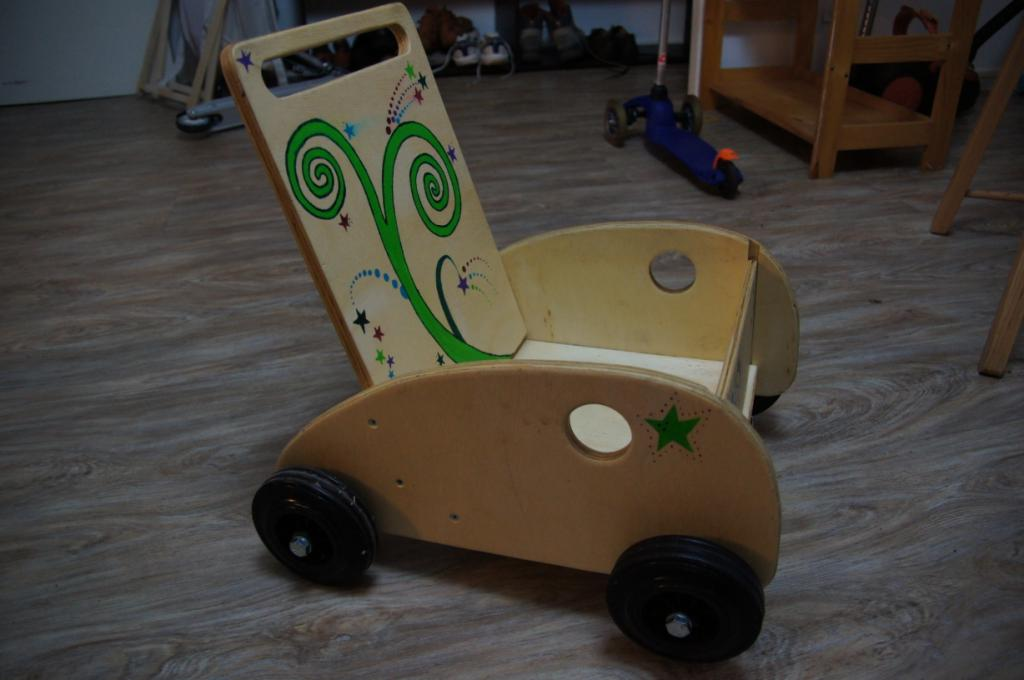
\includegraphics[width=0.6\linewidth]{images/chariot.jpg}

\end{center}



\section{Fournitures}

\subsection{Matériel}

\begin{tabular}{l l}
\begin{minipage}{0.5\linewidth}

\textbf{Contreplaqué multi-pli :}
 \begin{itemize}[label=$\bullet$]
\item en 15 mm :
\begin{itemize}
\item 30*40 cm
\item 30*30 cm
\item 45*20 cm ($\times$ 2)
\item 3*5 cm ($\times$ 10)
\end{itemize}
\item en 10 mm :
\begin{itemize}
\item 30.7*12.5 cm
\end{itemize}
\end{itemize}

\textbf{Roues :}
\begin{itemize}
\item Roues fixe (125 mm) ($\times$ 4)~\href{http://www.leroymerlin.fr/v3/p/produits/roue-fixe-sur-axe-pour-manutention-diametre-125-mm-e21277}{reférence}
\item Roues libres ($\times$ 2)~\href{http://www.leroymerlin.fr/v3/p/produits/roulette-pivotante-a-platine-pour-ameublement-diametre-50-mm-e21285}{reférence}
\end{itemize}
\end{minipage}
&
\begin{minipage}{0.5\linewidth}
\textbf{Autre :}
\begin{itemize}
\item Tube acier 7.5 cm * 14 mm (intérieur 12 mm) ~\href{http://www.leroymerlin.fr/v3/p/produits/tube-rond-lisse-en-acier-brut-l1m-x-ep0-1cm-d1-4cm-e17176}{reférence}
\item Vis M10 * 12 cm ($\times$ 4)
\item Écrou M10 avec frein ($\times$ 4)
\item Vis xxx ($\times$ 16)
\item Rondelle 30mm (intérieur 15mm) ($\times$ 4)
\item Rondelle 20mm (intérieur 11mm) ($\times$ 8)
\item Peintures
\item Vernis
\end{itemize}
\end{minipage}
\end{tabular}

\subsection{Prix}

\begin{tabular}{|l|c|}
\hline
Bois & $\sim$ 20\texteuro \\
Roues & $\sim$ 20\texteuro \\
Quincaillerie & $\sim$ 10\texteuro \\
Vernis & $\sim$ 5\texteuro \\
\hline
\hline
Total & $\sim$ 55\texteuro \\
\hline
\end{tabular}

\vspace{2mm}
Prix de vente neuf : $\sim$ 90\texteuro

\newpage

\section{Outillage}

\begin{multicols}{2}
\begin{itemize}
\item Serre-joints
\item Scie circulaire
\item Scie sauteuse
\item Scie cloche (30mm \& 50mm)
\item Embout à chanfreiner
\item Forêt à bois (1.5mm, 10mm \& 15mm)
\item Papier abrasif (grain 80 \& 120)
\item Pinceau pour vernis
\end{itemize}
\end{multicols}

\section{Pièces}
\subsection{En 15 mm d'épaisseur}
\begin{figure}[!h]
\captionsetup[subfigure]{labelformat=empty}
\subfloat[Pièce 1]{
\begin{tikzpicture}[scale=0.15]
    \draw[rounded corners=10] (0,0) -- (0,40) -- (30,40) -- (30,0);
    \draw (0,0) -- (30,0);
    \draw[color=gray,very thin,dashed] (4,36.5) circle (1.5); 
    \draw[color=gray,very thin,dashed] (26,36.5) circle (1.5);
    \draw (4,38) arc (90:270:1.5cm);
    \draw (26,38) arc (90:-90:1.5cm);
    \draw (4,38) -- (26,38);
    \draw (4,35) -- (26,35);
    
    \draw[<->] (0,-2) -- (30,-2) node [midway, below] {30cm};
    \draw[<->] (-2,0) -- (-2,40) node [ rotate=90, midway, above] {40cm};
    
    \draw[<->] (0,42) -- (4,42) node [midway, above] {4cm};    
    \draw[<->] (32,38) -- (32,35) node [ rotate=90, midway, below] {3cm};
  \end{tikzpicture}
  }
\subfloat[Pièce 2]{
\begin{tikzpicture}[scale=0.15]
    \draw (0,0) rectangle (30,30);
      
    \draw[<->] (0,-2) -- (30,-2) node [midway, below] {30cm};
    \draw[<->] (-2,0) -- (-2,30) node [ rotate=90, midway, above] {30cm};
  \end{tikzpicture}
  }
  
\subfloat[Pièce 3]{
\begin{tikzpicture}[scale=0.15]
    \draw[color=gray,very thin,dashed] (0,0) rectangle (45,20);
    
    \draw[name path=arc1] (0,10) arc (0:-90:-10cm);
	\draw (0,3) -- (0,10);
    \draw (0,3) arc (180:270:3cm);
	\draw (3,0) -- (42,0);
    \draw (42,0) arc (270:360:3cm);
    \draw (10,20) .. controls (25,20) and (45,10) .. (45,3);
    
    
    \path[name path=line1] (5,3) -- (5,20);
    \path[name path=line2] (6.1,3) -- (6.1,20);
    
    \path [name intersections={of=arc1 and line1}];
    
	\draw (intersection-1) -- (5,3);
	\draw (5,3) -- (6.1,3);
	
	 \path [name intersections={of=arc1 and line2}];
	 
	\draw (intersection-1) -- (6.1,3);
    
    
    \draw (14,14) circle (2.5);
    \fill (14,14) circle (0.1) node[below] {\tiny (14,14)};
    \draw[<->] (11,11) -- (16.5,11) node [midway, below] {\tiny 5cm};
    
	%vis
    \fill (11,3.5) circle (0.2) node[above] {\tiny (11,3.5)};
    \fill (27,3.5) circle (0.2) node[below] {\tiny (27,3.5)};
    \fill (31,6.5) circle (0.2) node[below] {\tiny (31,6.5)};
    \fill (33,12.5) circle (0.2) node[below] {\tiny (33,12.5)};
	    
	    
    \draw (6.5,1.5) circle (0.75) node[right] {\tiny (6.5,1.5)};
    \draw (40,1.5) circle (0.75) node[above] {\tiny (40,1.5)};
      
    \draw[<->] (0,22) -- (5,22) node [midway, above] {5cm};  
    \draw[<->] (5,22) -- (6,22) node [midway, below] {\tiny 11mm};       
      
    \draw[<->] (0,-2) -- (45,-2) node [midway, below] {45cm};
    \draw[<->] (-2,0) -- (-2,20) node [ rotate=90, midway, above] {20cm};
    \draw[<->] (4.5,0) -- (4.5,3) node [ rotate=90, midway, above] {\tiny 3cm};
  \end{tikzpicture}
  }
\subfloat[Pièce 4]{
\begin{tikzpicture}[scale=0.15]
    \draw (0,0) rectangle (5,3);
    
    \fill (1,1.5) circle (0.2);
    \fill (4,1.5) circle (0.2);
    
    \draw (2.5,1.5) circle (0.75);
    
    \draw[<->] (0,4) -- (1,4) node [midway, above] {\tiny 1cm};
    \draw[<->] (4,4) -- (5,4) node [midway, above] {\tiny 1cm};
    \draw[<->] (6,0) -- (6,1.5) node [ rotate=90, midway, below] {\tiny 1.5cm};
      
    \draw[<->] (0,-2) -- (5,-2) node [midway, below] {5cm};
    \draw[<->] (-2,0) -- (-2,3) node [ rotate=90, midway, above] {3cm};
  \end{tikzpicture}
  }
\end{figure}

\subsection{En 10 mm d'épaisseur}
\begin{figure}[!h]
\captionsetup[subfigure]{labelformat=empty}
\subfloat[Pièce 5]{
\begin{tikzpicture}[scale=0.1]
    \draw (0,0) rectangle (30.7,12.5);
      
    \draw[<->] (0,-2) -- (30.7,-2) node [midway, below] {30.7cm};
    \draw[<->] (-2,0) -- (-2,12.5) node [ rotate=90, midway, above] {12.5cm};
  \end{tikzpicture}
  }
\end{figure}

\newpage

\section{Fabrication}

\subsection{Conseils}
\begin{itemize}
\item Afin d'éviter que le bois n'éclate, pensez à utiliser des planches sacrificielles (surtout pour les trous).
\item Maintenez toujours votre planche bien plaqué contre son support à l'aire de \href{http://www.leroymerlin.fr/v3/p/produits/serre-joint-1-main-dexter-300-mm-e51423}{serre-joints}.
\item Utilisez un rail de guidage pour toutes les lignes droites (une \href{http://www.leroymerlin.fr/v3/p/produits/regle-avec-embout-nespoli-150-cm-e67206}{règle} avec des \href{http://www.leroymerlin.fr/v3/p/produits/lot-de-serre-joints-a-cadre-5-mm-e51365}{serre-joints} suffisent).
\end{itemize}

\subsection{Consignes}
\begin{enumerate}
\item Découper les planches 1 et 2 aux dimensions ci-dessus à l'aide d'une scie circulaire.
Faire attention à ce que les deux planches aient exactement la même largeur (30cm).
Adoucir les coins supérieurs de la pièce 1.
\item Dans la pièce 1, percer les trous de 30mm avec une scie cloche, finir l'ouverture avec une scie sauteuse, ou une scie à chantourner.
\item Reporter le contour de la pièce 3 sur deux nouvelles planches.
Afin d'avoir exactement la même forme, maintenir les deux planches 3 ensemble à l'aide de serre-joints.
Découper le contour à la scie sauteuse (ou à la scie à ruban).
\item Percer les trous de 50mm à la scie cloche.
\item Faire une rainure de 11mm dans les deux pièces 3 (vers l'intérieur du chariot) à la défonceuse en déplaçant progressivement le guide linéaire, ou à la scie circulaire (dans ce cas il faut faire la rainure sur toute la hauteur).
\item Percer les pré-trous en 1.5mm, puis les chanfreiner (depuis l'extérieur).


\item[???] Coller ou visser les rectangles (pièces 4)
\item Percer les 4 trous de 15mm à l'aide d'une perceuse à colonne.
\item Découper 4 bouts de tube, pour la longueur (x) reporter vous au schéma suivant :

\begin{figure}[!h]
\captionsetup[subfigure]{labelformat=empty}
\subfloat[Longueur du tube ($x$)]{
\begin{tikzpicture}[scale=0.5]
   \pgfmathsetmacro{\wrondelle}{0.1}%
\pgfmathsetmacro{\hrondelle}{2}%
\pgfmathsetmacro{\erondelle}{0.4}%
\pgfmathsetmacro{\xrondelle}{-\wrondelle}%

\pgfmathsetmacro{\xrondellebis}{4.5}%
\pgfmathsetmacro{\erondellebis}{0.5}%
\pgfmathsetmacro{\wrondellebis}{0.2}%
\pgfmathsetmacro{\wrondellebis}{0.2}%
\pgfmathsetmacro{\hrondellebis}{2.6}%
\pgfmathsetmacro{\xroue}{\xrondellebis+\wrondellebis}%
\pgfmathsetmacro{\wroue}{4}%
\pgfmathsetmacro{\hroue}{12}%

\pgfmathsetmacro{\xrondelleter}{\xroue+\wroue}%
\pgfmathsetmacro{\wrondelleter}{0.1}%
\pgfmathsetmacro{\hrondelleter}{2}%
\pgfmathsetmacro{\erondelleter}{0.5}%

\pgfmathsetmacro{\xtvis}{\xrondelleter+\wrondelleter}%
\pgfmathsetmacro{\wtvis}{1}%
\pgfmathsetmacro{\htvis}{1.5}%


\pgfmathsetmacro{\xvis}{-1.5}%
\pgfmathsetmacro{\wvis}{\xtvis-\xvis}%
\pgfmathsetmacro{\hvis}{0.8}%

\pgfmathsetmacro{\xtube}{0}%
\pgfmathsetmacro{\etube}{0.1}%
\pgfmathsetmacro{\wtube}{4.5+\wrondellebis+\wroue-0.2}%
\pgfmathsetmacro{\htube}{1.4}%


    \filldraw (\xrondelle,-\hrondelle/2)  rectangle +(\wrondelle,\hrondelle);
	\filldraw[white,draw=black] (\xrondelle,-\hrondelle/2+\erondelle)  rectangle +(\wrondelle,\hrondelle-2*\erondelle);

    %Pièces 4
	\draw[pattern=north west lines] (0,-1.5) rectangle +(1.5,3);
	 \filldraw[fill=white, draw=black] (0,0.8) rectangle +(1.5,-1.6);
	\draw [pattern=north east lines](1.5,-1.5) rectangle +(1.5,3);
	 \filldraw[fill=white, draw=black] (1.5,0.8) rectangle +(1.5,-1.6);
	\draw[<-] (0.75,2) -- (0.75,3) node [rotate=90,above] {\tiny Pièce 4}; 
	\draw[<-] (2.25,2) -- (2.25,3) node [rotate=90,above] {\tiny Pièce 4}; 
	
	%Pièce 3
    \draw[pattern=north west lines] (3,1.5) -- (3,5) .. controls (4,6) and (3.5,4) .. (4.5,5) --  (4.5,-1.5) -- (3,-1.5);
	 \filldraw[fill=white, draw=black] (3,0.8) rectangle +(1.5,-1.6);
	\draw[<-] (3.75,5.5) -- (3.75,6.5) node [rotate=90,above] {\tiny Pièce 3}; 
    
    %rondelle
    \filldraw (\xrondellebis,-\hrondellebis/2)  rectangle +(\wrondellebis,\hrondellebis);
	\filldraw[white,draw=black] (\xrondellebis,-\hrondellebis/2+\erondellebis)  rectangle +(\wrondellebis,\hrondellebis-2*\erondellebis);
    
    %roue
    \draw[dashed,gray] (\xroue,-\hroue/2)  rectangle +(\wroue,\hroue);
    \draw (\xroue,-0.8)  rectangle +(\wroue,1.6);
    \draw[<->] (\xroue,-\hroue/2-0.2) -- (\xroue+\wroue,-\hroue/2-0.2) node [midway, below] {\tiny largeur roue};
    \coordinate (A) at (\xroue,0.8);
    \draw [pattern=north east lines] (\xroue,0.8)-- +(0,1)
		 .. controls (\xroue,2.5) and (\xroue+\wroue/4,2)
 .. (\xroue+\wroue/4,\hroue/4 ) 
.. controls (\xroue+\wroue/4,\hroue/4 + 1) and (\xroue,\hroue/2-2) 
..  (\xroue,\hroue/2-1)
.. controls (\xroue,\hroue/2) and (\xroue +\wroue/3-1,\hroue/2) ..
 (\xroue +\wroue/3,\hroue/2)--(\xroue +2*\wroue/3,\hroue/2)
 .. controls  (\xroue +2*\wroue/3+1,\hroue/2) and (\xroue + \wroue,\hroue/2)
 .. (\xroue+\wroue,\hroue/2-1)
.. controls (\xroue+\wroue,\hroue/2-2)  and (\xroue+3*\wroue/4,\hroue/4 + 1) 
..  (\xroue+3*\wroue/4,\hroue/4 )
.. controls  (\xroue+3*\wroue/4,2)  and (\xroue+\wroue,2.5)
.. (\xroue+\wroue,1.8) -- (\xroue+\wroue,0.8) -- (\xroue,0.8);

\draw [pattern=north east lines] (\xroue,-0.8) -- +(0,-1)
		 .. controls (\xroue,-2.5) and (\xroue+\wroue/4,-2)
 .. (\xroue+\wroue/4,-\hroue/4 ) 
.. controls (\xroue+\wroue/4,-\hroue/4 - 1) and (\xroue,-\hroue/2+2) 
..  (\xroue,-\hroue/2+1)
.. controls (\xroue,-\hroue/2) and (\xroue +\wroue/3-1,-\hroue/2) ..
 (\xroue +\wroue/3,-\hroue/2)--(\xroue +2*\wroue/3,-\hroue/2)
 .. controls  (\xroue +2*\wroue/3+1,-\hroue/2) and (\xroue + \wroue,-\hroue/2)
 .. (\xroue+\wroue,-\hroue/2+1)
.. controls (\xroue+\wroue,-\hroue/2+2)  and (\xroue+3*\wroue/4,-\hroue/4 - 1) 
..  (\xroue+3*\wroue/4,-\hroue/4 )
.. controls  (\xroue+3*\wroue/4,-2)  and (\xroue+\wroue,-2.5)
.. (\xroue+\wroue,-1.8) -- (\xroue+\wroue,-0.8) -- (\xroue,-0.8);
    

	\draw[<-] (\xroue+\wroue/2,\hroue/2+0.5) -- (\xroue+\wroue/2,\hroue/2+1.5) node [rotate=90,above] {\tiny Roue};     
    
    %rondelle
     \filldraw (\xrondelleter,-\hrondelleter/2)  rectangle +(\wrondelleter,\hrondelleter);
	\filldraw[white,draw=black] (\xrondelleter,-\hrondelleter/2+\erondelleter)  rectangle +(\wrondelleter,\hrondelleter-2*\erondelleter);

	%tube
    \filldraw[fill=red!40!white, draw=red] (\xtube,-\htube/2) rectangle +(\wtube,\htube);
	\fill[red] (\xtube,-\htube/2) rectangle +(\wtube,\etube);
	\fill[red] (\xtube,\htube/2) rectangle +(\wtube,-\etube);
	
    \draw[<->] (0,-2) -- (\wtube,-2) node [midway, below left] { $x$ cm};
    \draw[>-<] (\wtube-0.1,-2) -- (\xrondelleter+0.1,-2) node [midway, below right] {\tiny 1-2 mm};

	%ecrou
    \draw[pattern=north east lines] (\xrondelle-\wtvis,-\htvis/2) rectangle +(\wtvis,\htvis);

	%vis
    \draw[pattern=north west lines] (\xtvis,-\htvis/2) rectangle +(\wtvis,\htvis);

	\filldraw[fill=white,draw=black,snake=zigzag, segment amplitude=1,segment length=3] (\xvis,-\hvis/2) -- (\xvis+\wvis,-\hvis/2) [snake=none] -- (\xvis+\wvis,\hvis/2)  [snake=zigzag, segment amplitude=1,segment length=3] -- (\xvis,+\hvis/2)  [snake=none] -- (\xvis,-\hvis/2) ;
	\fill[pattern=north west lines,snake=zigzag, segment amplitude=1,segment length=3] (\xvis,-\hvis/2) -- (\xvis+\wvis,-\hvis/2) [snake=none] -- (\xvis+\wvis,\hvis/2)  [snake=zigzag, segment amplitude=1,segment length=3] -- (\xvis,+\hvis/2)  [snake=none] -- (\xvis,-\hvis/2) ;
    
    
    
  \end{tikzpicture}
  }
\end{figure}

\item Assembler les différentes pièces en vissant un coté puis l'autre.
\item Mesurer l'écartement entre les rainures et ajuster les dimensions de la pièce 5 pour qu'elle puisse coulisser facilement (1mm de marge de chaque coté).
La découper à la scie circulaire.
\item Adoucir tous les bords au papier abrasif.
\item[Facultatif.] Ajouter une touche de peinture puis vernir.
\end{enumerate}

\section{Utilisation}

Pour l'apprentissage de la marche ne pas mettre les roues folles, le chariot doit aller uniquement en ligne droite.
Penser à ajuster le freinage à l'aide des boulons sur les différentes roues.

Une fois que l'enfant marche correctement, ajouter les roues folles pour plus de liberté.


\vfill
\hfill \small Document réalisé avec \LaTeX
\end{document}